\documentclass[11pt]{article}

\input{glyphtounicode}
\pdfgentounicode=1
\ifdefined\pdfinterwordspaceon
  \pdfinterwordspaceon
\fi

\usepackage[utf8]{inputenc}
\usepackage{cmap}
\usepackage[T1]{fontenc}
\usepackage{lmodern}
\usepackage{microtype}
\usepackage{amsmath,amssymb}
\usepackage{graphicx}
\usepackage{float}
\usepackage{booktabs}
\usepackage{array}
\usepackage{longtable}
\usepackage{enumitem}
\usepackage{xcolor}
\usepackage[font=small,justification=raggedright,singlelinecheck=false]{caption}
\usepackage{url}
\usepackage{indentfirst}
\usepackage{flafter}
\usepackage{placeins}
\usepackage{needspace}
% Temporary author-year citation mode for final manual reference verification.
% For arXiv numeric submission, switch back to:
% \usepackage[numbers,sort&compress]{natbib}
% \bibliographystyle{unsrtnat}
\usepackage[authoryear,round]{natbib}
\setlength{\bibsep}{2pt plus 0.3ex}
\usepackage[colorlinks=true,linkcolor=blue,citecolor=blue,urlcolor=blue]{hyperref}
\usepackage[nameinlink,capitalise,noabbrev]{cleveref}

% arXiv submission plan: primary cs.SE; cross-list cs.AI and cs.CL.
% Preferred license for this version: CC BY 4.0, unless a later publisher
% requires the arXiv default non-exclusive license.

\Urlmuskip=0mu plus 2mu\relax
\captionsetup[figure]{font=small,justification=raggedright,singlelinecheck=false}
\captionsetup[table]{font=small,justification=raggedright,singlelinecheck=false}
\captionsetup[longtable]{font=small,justification=raggedright,singlelinecheck=false}
\setlength{\textfloatsep}{6pt plus 2pt minus 2pt}
\setlength{\floatsep}{6pt plus 2pt minus 2pt}
\setlength{\intextsep}{7pt plus 2pt minus 2pt}
\setlength{\LTpre}{6pt plus 2pt minus 2pt}
\setlength{\LTpost}{6pt plus 2pt minus 2pt}
\setlength{\abovecaptionskip}{3pt plus 1pt minus 1pt}
\setlength{\belowcaptionskip}{1pt plus 1pt minus 1pt}
\setlength{\parskip}{0pt}
\frenchspacing
\raggedbottom
\newcolumntype{L}[1]{>{\raggedright\arraybackslash}m{#1}}
\newcolumntype{C}[1]{>{\centering\arraybackslash}m{#1}}
\setcounter{topnumber}{4}
\setcounter{bottomnumber}{2}
\setcounter{totalnumber}{5}
\renewcommand{\topfraction}{0.92}
\renewcommand{\bottomfraction}{0.75}
\renewcommand{\textfraction}{0.06}
\renewcommand{\floatpagefraction}{0.82}
\makeatletter
\setlength{\@fptop}{0pt}
\setlength{\@fpsep}{6pt plus 1fil}
\setlength{\@fpbot}{0pt plus 1fil}
\renewcommand\section{\@startsection{section}{1}{\z@}%
  {1.75ex}%
  {0.82ex}%
  {\normalfont\Large\bfseries}}
\renewcommand\subsection{\@startsection{subsection}{2}{\z@}%
  {1.50ex}%
  {0.72ex}%
  {\normalfont\large\bfseries}}
\renewcommand\paragraph{\@startsection{paragraph}{4}{\z@}%
  {0.90ex}%
  {-0.75em}%
  {\normalfont\normalsize\bfseries}}
\makeatother
\newcommand{\PostTableHeadingSpace}{\FloatBarrier\vspace{-0.35\baselineskip}}
\newcommand{\PostFigureHeadingSpace}{\FloatBarrier\vspace{-0.35\baselineskip}}
\newcommand{\PostReferencesSpace}{\FloatBarrier\vspace{-0.28\baselineskip}}

\title{Beyond Prompting: Harness Engineering for Enterprise LLM Agents}

\author{%
  Joongho Ahn\\
  AI Leadership Research Center\\
  \texttt{joongho@ceoai.kr}
  \and
  Moonsoo Kim\thanks{Corresponding author.}\\
  AI Leadership Research Center\\
  \texttt{mskim@ceoai.kr}
}

\date{}

\begin{document}

\maketitle

\begin{abstract}
Enterprise large language model (LLM) applications are often first explored as prototypes whose behavior is carried by prompts and retrieval context. These prototypes can demonstrate useful interactions, but productization adds requirements for source boundaries, entity routing, answer contracts, and reproducible traces. We present a harness-engineering approach that reconstructs this prototype pattern into a traceable LLM-agent architecture. The method moves deterministic behavior into code, manifests, schemas, and validation artifacts, while source-backed claims remain the authority for runtime answers. We apply the approach to a public-data reference slice of five Korean corporate groups, 25 listed companies, and 113 source-backed runtime claims. The baseline passes 30/30 fixed validation-scenario contract checks, including source-reference resolution, trace preservation, answer-structure checks, and user-facing output hygiene. Runtime interface checks further exercise live filing, market, and news connections; in a separate 14-scenario orchestration check, caching and parallel source collection reduce mean measured latency from 2008.57ms to 171.14ms. The result is a reusable engineering pattern for turning exploratory enterprise LLM prototypes into auditable and extensible applications with versioned source, control, and validation artifacts.
\end{abstract}


\section{Introduction}

Enterprise large language model (LLM) applications are often explored first as demonstrations: a system prompt, a set of retrieved documents, and a user interface that shows the intended interaction. We call a prototype prompt-dominant when important product behavior is encoded mainly as natural-language instructions or broad retrieval context, with code, data contracts, and validation artifacts still underdeveloped. Prompt-dominant development is useful for exploration and is related to vibe coding, a conversational AI-assisted software workflow popularized by Karpathy \citep{karpathy2025vibecoding,meske2025vibecoding}. Productization introduces a different requirement: each visible claim should be traceable to bounded sources, routed to the correct entity, regenerated under the same assumptions, and inspected through explicit artifacts. These concerns connect to prior work on hallucination and software-engineering controls for artificial intelligence (AI) systems \citep{ji2023hallucination,martinezfernandez2022seai,kreuzberger2023mlops}.

The study examines this transition through the reconstruction of an LLM-based investment briefing agent. The motivating prototype was developed during a ten-week AI leadership program hosted by CEO AI \citep{ceoai2026leadership}; the authors report the work under the AI Leadership Research Center affiliation associated with that program context. During the program, the authors built and demonstrated over ten exploratory AI product prototypes for executive- and client-facing scenarios, using Replit-hosted demonstrations to share interaction patterns with participants \citep{replit2026platform}. The investment-briefing prototype supplied useful interaction patterns, including mobile-first briefing cards, source links, voice-oriented flows, and follow-up questions. The prototype serves as motivating context for a reconstructed system with a different source, trace, and validation structure.

We propose a harness-engineering approach for converting a demonstration prototype into a traceable research system. In software engineering, a test harness refers to scaffolding code used to exercise lower-level code before the higher-level code that will ultimately invoke it is available \citep{isoiecieee2017vocabulary}. We extend the test-harness idea to enterprise LLM agents: the harness is the code-owned control layer around the model, responsible for source gates, routing rules, claim eligibility, answer contracts, trace logging, and validation. In the reconstructed architecture, manifests define what sources may be used, source-backed claims define what statements may enter runtime context, routing metadata binds questions to entities, answer contracts define the visible response, and traces record how the answer was assembled. Maintained wiki pages, following the LLM Wiki pattern, provide compact context while source manifests and source-backed claims remain authoritative \citep{karpathy2026llmwiki}.

The paper contributes a harness-engineering method for reconstructing prompt-dominant enterprise LLM prototypes into traceable LLM-agent architectures; a source-to-claim knowledge pipeline that separates raw documents, evidence records, runtime-eligible claims, maintained wiki context, and user-facing answers; a replaceable composition boundary that separates deterministic harness control from LLM phrasing; and a system-level validation design for checking traceability, routing, prompt-to-code migration, internal-output leakage prevention, runtime-interface behavior, and latency. We instantiate the method on a bounded public-data slice of five Korean corporate groups, 25 listed companies, and 113 source-backed runtime claims.

\section{Related Work}

This section reviews the research and engineering practices needed to turn LLM-agent prototypes into traceable enterprise systems. The organizing question is how an answer can be grounded, assembled, constrained, and validated before it is presented to the user.

\paragraph{RAG and traceability.}
Retrieval-augmented generation (RAG) combines language models with external documents to improve factual grounding and updateability \citep{lewis2020rag,gao2023rag}. Later work shows that retrieval must also be selective and checkable: self-reflective retrieval methods ask whether retrieval is needed and whether generation is supported \citep{asai2024selfrag}, while factuality metrics decompose long-form answers into atomic claims \citep{min2023factscore}. Retrieval selectivity and factual checkability are directly relevant to enterprise domains where disclosures, investor-relations (IR) materials, news, and regulatory filings change over time. Retrieval provides factual context, while traceability additionally requires source state, entity scope, and claim-level support. Retrieved passages may be stale, irrelevant, or mixed across entities, and fluent generation may still hallucinate \citep{ji2023hallucination}. Our approach treats RAG as one component inside a structured source-to-claim harness.

\paragraph{LLM agents and orchestration.}
Classical agent research emphasizes autonomy, interaction, and explicit system architecture \citep{wooldridge1995intelligent,jennings1998roadmap}. LLM agents extend the classical agent tradition through tool use, planning, search, and intermediate execution traces \citep{yao2023react,schick2023toolformer,wang2024surveyagents,acharya2025agentic}. Tool-use benchmarks further show that API selection and execution are engineering concerns as well as prompting concerns \citep{qin2024toolllm}. Recent applied work also reports multi-platform agent deployment and programmable agent runtime architectures \citep{ahn2025autonomous,walters2025eliza}. The present paper shifts the emphasis from multi-platform deployment to enterprise hardening: each answer must record which sources, tools, claims, and fallback paths shaped the final output.

Recent orchestration frameworks make agent engineering more concrete. AutoGen supports multi-agent conversation and coordination \citep{wu2024autogen}; LangChain Agents provide prebuilt tool-calling loops and LangGraph provides graph-based runtimes for stateful agents \citep{langchain2026agents,langchain2026langgraph}; and CrewAI organizes role-based agents, crews, and flows \citep{crewai2026software}. The proposed control layer is complementary to these frameworks: orchestration frameworks address how agents are composed and executed, while the pattern studied here addresses whether each produced answer is grounded in source manifests, claim records, output contracts, and validation traces. In deployment, it can surround a LangGraph, CrewAI, AutoGen, or LangChain-agent workflow.

\paragraph{Prompt engineering and prototyping.}
Prompt engineering became important because large language models can perform new tasks from natural-language instructions and in-context examples \citep{brown2020language,liu2023pretrain}. Prompt engineering also entered broader academic and practitioner discourse as users learned to shape model outputs through prompt design \citep{giray2023prompt}. Techniques such as chain-of-thought prompting further showed that changing the prompt can substantially change reasoning behavior \citep{wei2022chain}. Vibe coding extends prompt design from isolated task instructions to an iterative development workflow in which software behavior is co-created through natural-language dialogue with AI tools \citep{karpathy2025vibecoding,meske2025vibecoding,malamas2025vibecoding}. Prompting and vibe-coding techniques are valuable for early exploration and are one reason prototype systems can be built quickly. The transition addressed by the present paper appears when prompts stop being only task instructions and become the place where source policy, entity routing, answer structure, data freshness rules, and user-interface behavior are implicitly stored. At that point, the system becomes prompt-dominant: effective for exploration, while audit, replay, and transfer require stable responsibilities to be moved into explicit artifacts.

\paragraph{Programmable LLM pipelines.}
Several frameworks argue that LLM applications should be programmed, tested, and optimized with explicit software abstractions. Demonstrate-Search-Predict and DSPy represent language-model pipelines as composable declarative programs \citep{khattab2022demonstrate,khattab2024dspy}; the DSPy project repository is also cited as a software artifact \citep{stanfordnlp2026dspysoftware}. LMQL and Guidance treat model interaction as controlled execution \citep{beurerkellner2023lmql,guidance2026software}; and Instructor uses typed schemas to constrain outputs \citep{instructor2026software}. Runtime guardrail systems such as NeMo Guardrails similarly show how user-defined rails can control conversational behavior independently of the underlying model \citep{rebedea2023nemo}. Autoresearch illustrates how improvement can be organized as repeatable experiments with explicit logs \citep{karpathy2026autoresearch}. Our contribution is to apply the programming-oriented philosophy at the product-architecture level: routing, source eligibility, claim promotion, answer planning, follow-up filtering, and internal-output leakage prevention are implemented as code and data structures.

\paragraph{LLM Wiki and knowledge management.}
Karpathy's LLM Wiki pattern proposes a maintained markdown knowledge layer between raw sources and query-time answers \citep{karpathy2026llmwiki}. In that pattern, the LLM helps maintain a persistent wiki of entity pages, topic summaries, links, contradictions, and logs, reducing repeated synthesis from the same raw documents. The pattern is useful for research and business settings where knowledge accumulates over time. The proposed system adopts the maintained-knowledge idea while assigning authority to source manifests and source-backed claims: raw source manifests and source-backed claims remain the source of truth, and the LLM Wiki is compiled as a concise context layer for humans and models.

\paragraph{System validation and evaluation.}
Software-engineering research on AI-based systems emphasizes that production AI depends on data management, testing, lifecycle controls, monitoring, and assurance artifacts in addition to model performance \citep{martinezfernandez2022seai,ashmore2021assuring}. Machine learning operations (MLOps) research similarly treats operationalization as a lifecycle concern that spans the full system lifecycle \citep{kreuzberger2023mlops}. RAG evaluation frameworks measure faithfulness, answer relevance, context precision, and context recall \citep{es2023ragas,saadfalcon2024ares}, while broader benchmark work supports multi-scenario evaluation \citep{liang2023helm}. Practitioner tools also support prompt, model, and application regression checks \citep{promptfoo2026software}. The present paper uses system validation suited to a pre-commercial research prototype before customer logs are available. The focus is whether fixed scenarios preserve source-backed claims, entity routing, trace contracts, answer structure, interface status, and latency.

\section{Method}

The method reconstructs a prompt-dominant LLM prototype into a traceable LLM-agent architecture. The language model remains responsible for language composition, and source selection, entity routing, claim eligibility, answer structure, trace logging, and validation are represented as explicit artifacts.

\subsection{Architecture Overview}

\vspace{0.35\baselineskip}

\begin{figure}[H]
    \centering
    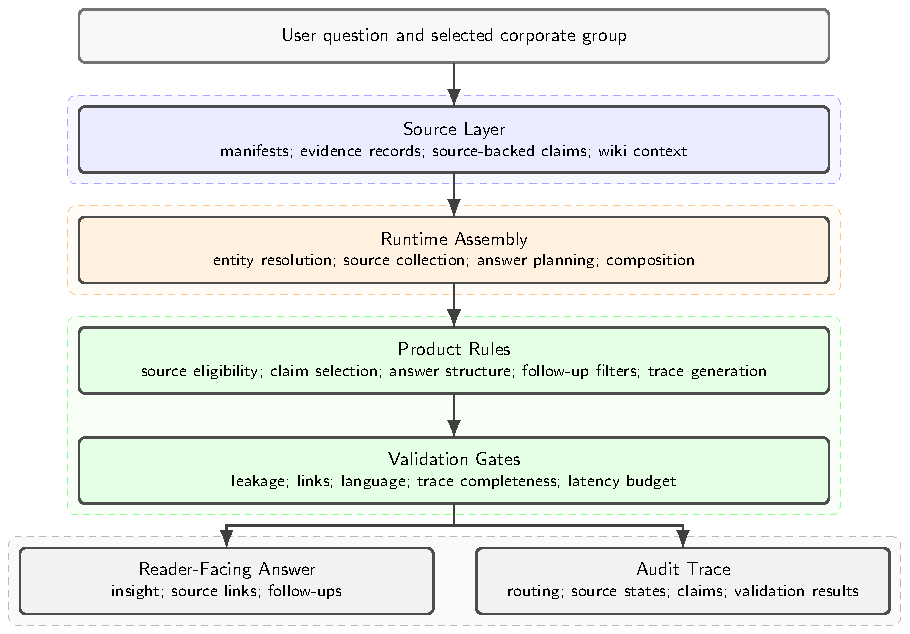
\includegraphics[width=0.95\linewidth,height=0.50\textheight,keepaspectratio]{figures/harness_architecture.pdf}
    \caption{Traceable LLM-agent harness. The architecture separates source authority, runtime assembly, product rules, validation gates, and two outputs: a reader-facing answer and an audit trace.}
    \label{fig:harness-architecture}
\end{figure}

The architecture in \Cref{fig:harness-architecture} starts from a user question and a selected Korean corporate group. The selected entity resolves aliases, market identifiers, filing identifiers, and source namespaces. The runtime returns a reader-facing answer and an audit trace. The trace records routing, source collection, claim selection, answer assembly, and validation, while the control layer manages source eligibility, answer structure, validation, and trace generation.

\subsection{Source-to-Claim Pipeline}

The system first registers raw materials as source manifests. A manifest records the corporate-group scope, company scope, source title, issuer, source category, public URL or filing identifier, local path when available, checksum, rights policy, selection rule, and runtime use policy. Manifest registration prevents the knowledge base from becoming an unbounded document folder.

Documents that pass the source gate are extracted or manually reviewed. Evidence records store file hashes, extracted-text hashes, and evidence locations such as page or line references when available. The system then produces claim candidates. A candidate becomes runtime-eligible only when it is promoted into a source-backed claim: an atomic statement linked to a source manifest, evidence record, claim type, company scope, use policy, and verification state. The claim layer is a key design boundary in our architecture. The model may use source-backed claims as bounded context; related documents require claim promotion before they authorize factual statements.

\subsection{Knowledge Layer and Product Rules}

Following the LLM Wiki pattern, the system maintains markdown knowledge pages that sit between raw source documents and runtime answers \citep{karpathy2026llmwiki}. In our implementation, the maintained knowledge layer is compiled from reviewed artifacts and functions as a context layer. The maintained knowledge layer gives humans and LLMs concise context; source manifests and source-backed claims remain authoritative.

The reconstruction also moves product rules out of the prompt. Entity routing, source eligibility, runtime source state, claim selection, answer-section planning, follow-up filtering, output validation, internal-trace separation, and stage-gate checks are implemented as code, manifests, schemas, and validators. The prompt is kept short and policy-oriented. The prompt-to-code migration is intended to reduce the burden on the model and make diagnostic boundaries easier to locate; direct measurement of prompt-complexity reduction is left to later work.

\subsection{Runtime Answer Assembly}

At runtime, the control layer resolves the selected corporate group and company, collects filing, market, news, wiki, and claim context, builds an answer plan, generates the visible response, validates the output contract, and records the trace. The process trace records tool and source states such as live, local, fallback, fixture, or error. The answer-assembly trace records routing, source collection, claim selection, answer planning, and validation-check results.

The visible answer follows an insight-first contract. It must begin with a reader-facing interpretation, then provide supporting signals, risks or contradictions, source links, and follow-up questions. Follow-up questions are treated as part of the output contract: the reference implementation generates them with a deterministic topic-conditioned builder, and validation checks that enough customer-facing follow-ups are present and free of generic or internal-review wording. Internal artifacts such as claim identifiers, raw trace JSON, and API status labels are reserved for the internal review interface.

\subsection{Reference Implementation}
\label{sec:implementation-details}

The reference implementation is a TypeScript application with JavaScript Object Notation (JSON) source, claim, scenario, and evaluation artifacts. The public release reference is recorded as a placeholder repository citation and should be replaced with the final GitHub URL and submission commit hash before submission \citep{ahnkim2026advisorrepo}. The baseline reported in the paper uses a deterministic, schema-checked composer for fixed validation scenarios and runtime-interface tests. The composer is a rule-based template engine that fills validated answer sections from selected source-backed claims using no generative model call. This baseline fixes the system contract and separates validation of the control layer from model sampling effects.

The architecture treats composition as a replaceable boundary. Source selection, entity routing, claim eligibility, answer-section planning, follow-up filtering, trace creation, and validation are owned by the control layer and remain independent of a particular LLM. A live LLM may be attached at the composition boundary to phrase a structured answer; its output must pass the same output contract. If the live output is unavailable or invalid, the runtime falls back to the deterministic composer. Future live-LLM comparisons can be reported as separate traces with provider, model identifier, API date, temperature or default-temperature policy, token limit, prompt version, and schema version.

\subsection{Validation and Trace Contracts}

A target slice enters the paper baseline after it passes source, claim, routing, answer, trace, and latency checks. Fixed validation-scenario tests verify expected claim coverage, entity routing, trace integrity, internal-trace leakage prevention, follow-up quality, and output structure. Live API interface tests verify filing, market, and news interfaces and record connectivity as a runtime state. Review packets collect the visible answer, user-facing source links, follow-up questions, selected claims, and trace paths so that the reader evidence surface and the internal audit trail can be inspected separately before any later expert review.

Validation is implemented as three visible families of checks. Leakage checks block internal claim identifiers, raw trace JSON, API diagnostics, fixture labels, and internal-only status text from the reader-facing answer. Link checks require cited sources and follow-ups to resolve to source packages, public locators, or documented fallback states. Language checks enforce the insight-first answer structure and block recommendation-style phrasing such as buy, sell, or target-price instructions.

The trace contract that supports these gates is summarized in \Cref{tab:runtime-trace-example}. The trace contract is a method artifact: it records how a visible answer was assembled while keeping internal details out of the reader-facing answer.

\vspace{-0.35\baselineskip}
\begin{table}[H]
    \centering
    \caption{Runtime trace contract summary.}
    \label{tab:runtime-trace-example}
    \footnotesize
    \setlength{\tabcolsep}{4pt}
    \renewcommand{\arraystretch}{1.12}
    \begin{tabular}{@{}C{0.18\linewidth}
                    L{0.31\linewidth}
                    L{0.22\linewidth}
                    L{0.17\linewidth}@{}}
        \toprule
        \multicolumn{1}{C{0.18\linewidth}}{Runtime stage} & \multicolumn{1}{C{0.31\linewidth}}{Recorded value} & \multicolumn{1}{C{0.22\linewidth}}{Trace evidence} & \multicolumn{1}{C{0.17\linewidth}}{User visibility} \\
        \midrule
        \shortstack{Entity\\routing} & Selected group, company ID, and aliases & Routing and company metadata & Selected label \\
        \shortstack{Source\\collection} & DART, market, news, wiki, and claim states & Process trace with source state & Source links and freshness labels \\
        \shortstack{Claim\\selection} & Source-backed claim IDs and types & Answer-assembly trace & Hidden \\
        \shortstack{Answer\\planning} & Answer sections and follow-up filters & Output-contract result & Structured answer and follow-ups \\
        \shortstack{Output\\validation} & Leakage, link, language, and latency checks & Validation trace and JSON path & Internal review \\
        \bottomrule
    \end{tabular}
\end{table}
\vspace{-0.45\baselineskip}

\PostTableHeadingSpace
\section{Data and Knowledge Construction}

The reference implementation uses a bounded public-data slice to document how enterprise source material is turned into runtime knowledge. The section describes the company selection rule, source registration process, claim-promotion layer, and runtime claim set used for the paper baseline. The generated mobile briefing surface in \Cref{fig:ui-mobile-main} shows this data layer in product form: the selected state aligns the header price, news, stock, and filing-linked financial cards with the selected corporate group, and the selector callout shows the same surface switching across five groups.

\begin{figure}[H]
    \centering
    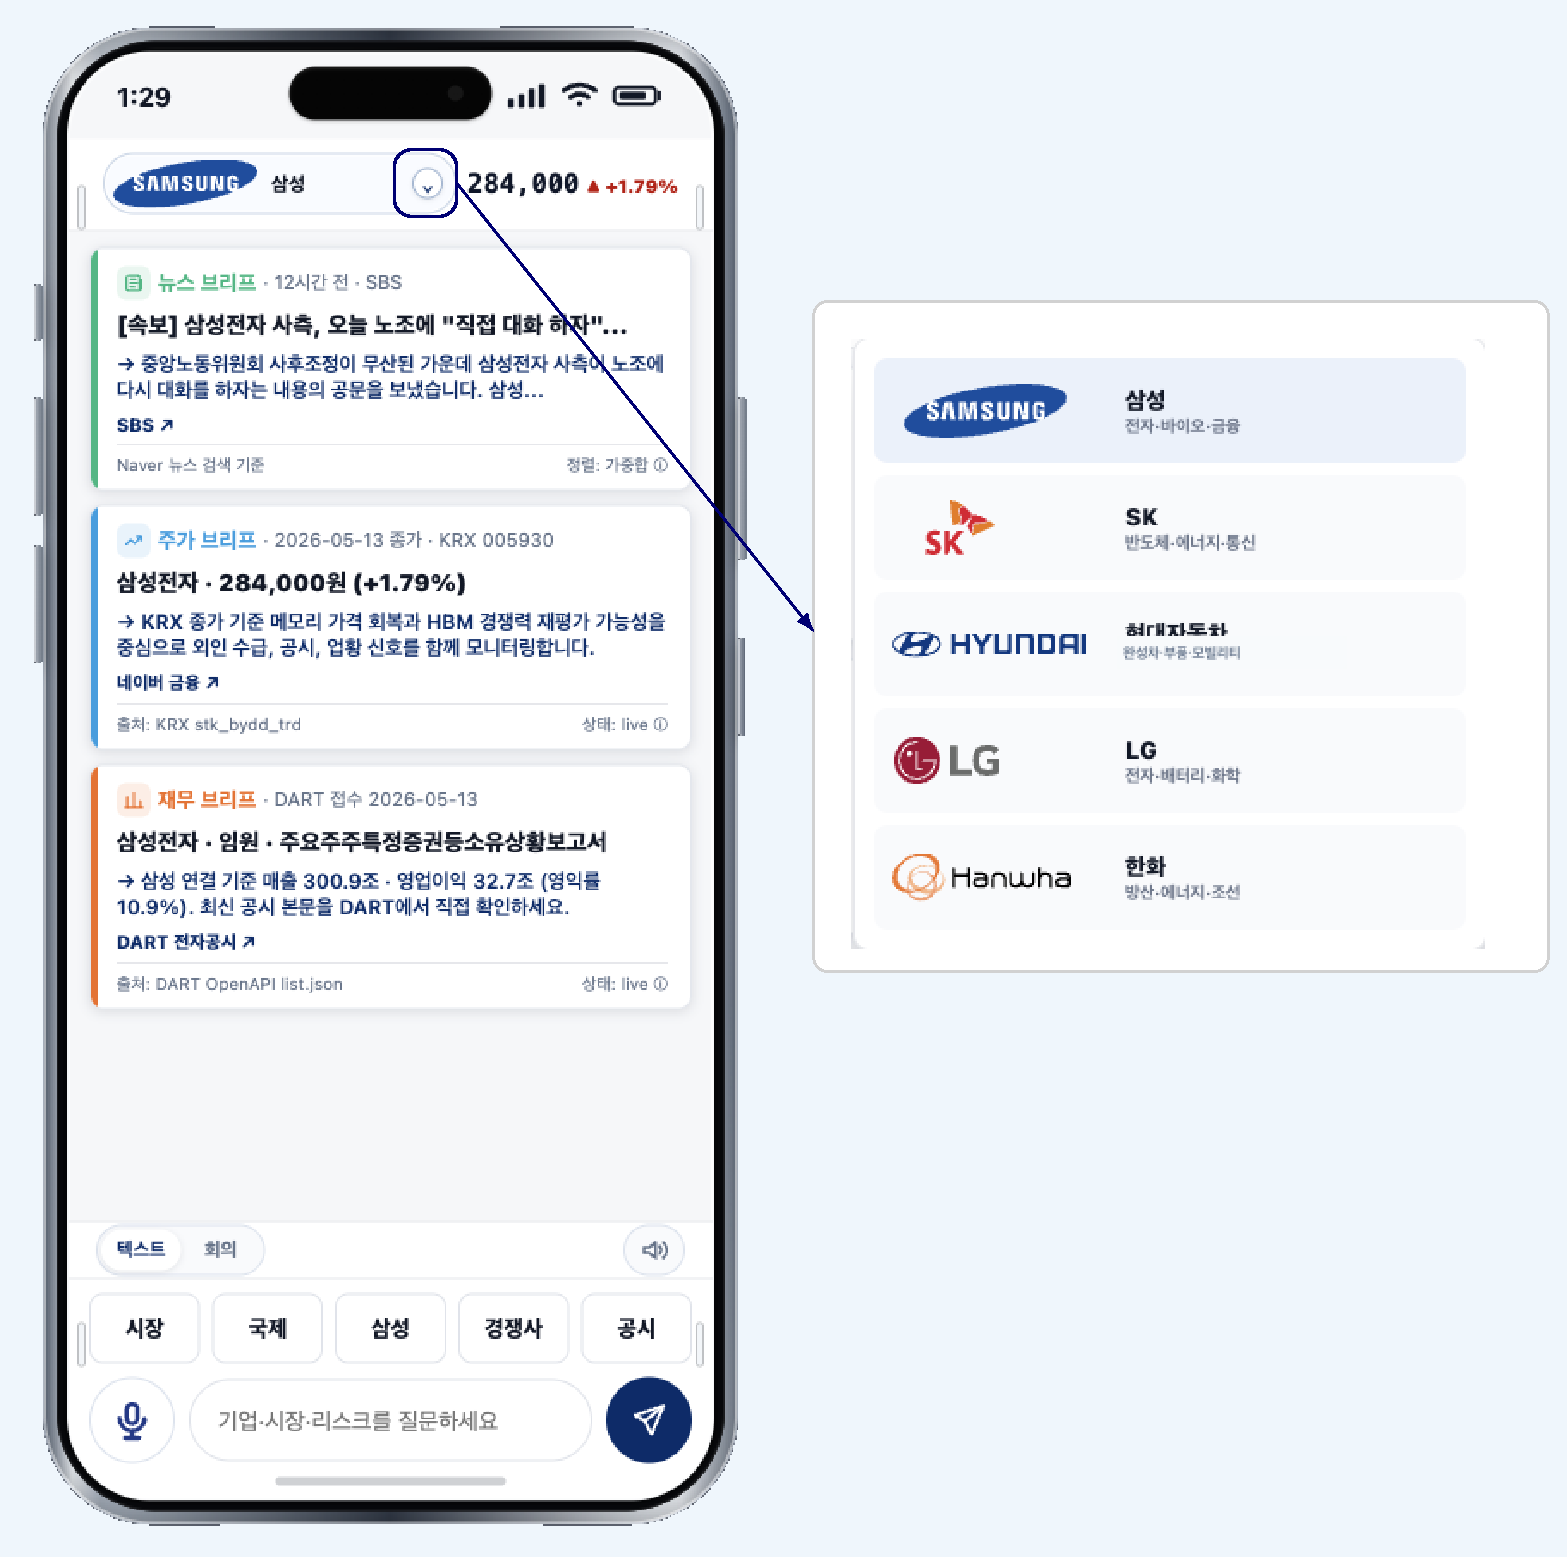
\includegraphics[width=0.95\linewidth]{figures/ui_mobile_main_ko_callout.pdf}
    \caption{Mobile main-screen briefing surface with selector callout. The selected Samsung state illustrates the shared interface, including news, stock, and filing-linked financial cards; the callout shows that the same surface switches among the five corporate groups.}
    \label{fig:ui-mobile-main}
\end{figure}

\subsection{Reference Company Slice}

The current slice covers five Korean corporate groups and five listed companies per corporate group. In this paper, a Korean corporate group refers to the corporate-group designation unit used by the Fair Trade Commission. The corporate-group boundary follows the 2026 ranking by fair-value assets in the official Fair Trade Commission designation results: Samsung, SK, Hyundai Motor, LG, and Hanwha form the top-five corporate-group set after Hanwha entered fifth place \citep{ftc2026businessgroups}. The ranking provides a reproducible sampling rule for the reference slice, independent of investment-quality assessment.

Within each corporate group, the five listed companies are selected by a fixed reference-slice policy. The policy prioritizes listed companies with stable KRX and OpenDART identifiers, corporate-group representativeness, sector diversity, comparability across corporate groups, public-source availability, claim-promotion feasibility, investor-facing relevance, and scope control. The five corporate groups test transfer across different source structures: affiliate-level IR pages, DART filings, holding-company materials, market-data interfaces, and news-search interfaces. The controlled 25-company slice supports routing and transferability tests while keeping source eligibility auditable. The selected companies and coverage focus used for the reference slice are defined in \Cref{tab:reference-slice-selection}.

\begin{table}[H]
    \centering
    \caption{Reference-slice company selection. Each corporate group contributes five listed companies selected for identifier readiness, representativeness, sector diversity, comparability, and source availability.}
    \label{tab:reference-slice-selection}
    \footnotesize
    \setlength{\tabcolsep}{4pt}
    \setlength{\extrarowheight}{1pt}
    \renewcommand{\arraystretch}{1.32}
    \begin{tabular}{@{}C{0.16\linewidth}
                    L{0.47\linewidth}
                    L{0.29\linewidth}@{}}
        \toprule
        \multicolumn{1}{C{0.16\linewidth}}{Corporate group} & \multicolumn{1}{C{0.47\linewidth}}{Selected listed companies} & \multicolumn{1}{C{0.29\linewidth}}{Coverage focus} \\
        \midrule
        Samsung & Samsung Electronics; Samsung SDI\newline Samsung C\&T; Samsung Biologics\newline Samsung Electro-Mechanics & Memory, battery, construction, bio, components \\
        \addlinespace[0.50em]
        SK & SK Hynix; SK Innovation; SK Inc.\newline SK Telecom; SK Square & Memory, energy, holding, telecom, ICT investment \\
        \addlinespace[0.50em]
        Hyundai Motor & Hyundai Motor; Kia; Hyundai Mobis\newline Hyundai Glovis; Hyundai Rotem & OEMs, parts, logistics, defense/rail \\
        \addlinespace[0.50em]
        LG & LG Electronics; LG Chem\newline LG Energy Solution; LG Innotek\newline LG Uplus & Electronics, materials, battery, components, telecom \\
        \addlinespace[0.50em]
        Hanwha & Hanwha Corp.; Hanwha Systems\newline Hanwha Aerospace; Hanwha Ocean\newline Hanwha Solutions & Holding, aerospace, energy, systems, shipbuilding \\
        \bottomrule
    \end{tabular}
\end{table}

Sources include issuer IR materials, earnings presentations, annual and periodic filings, governance documents, public filing URLs, market-data interfaces, and news-search interfaces. The raw public inputs used by the implementation fall into four practical classes: DART filings, issuer IR materials, KRX market rows, and news-search results. For Korean filing, market, and news data, the implementation uses OpenDART, Korea Exchange (KRX) OPEN API, and NAVER News Search as interface sources \citep{opendart2026api,krx2026openapi,naver2026newssearch}. DART and IR materials provide most promoted financial and corporate claims in the paper baseline, while KRX and news-search inputs provide runtime market and news signals that are linked, checked, and traced separately. A source is included in the runtime layer when it supports a claim class, fixed validation scenario, runtime feature, or onboarding requirement. Files discovered during official-site scans are recorded for provenance and are promoted into runtime use when they support a specific claim or validation need.

The broader source ledger is larger than the 25-company runtime slice. The ledger records company-level source metadata, public locators, local artifact pointers when available, provenance fields, selection reasons, and document-type classifications across the collected public materials. Source-inventory counts function as audit artifacts. Runtime answers depend on promoted claims, source manifests, and validation gates.

\subsection{Manifest and Claim Records}

Each source is first represented as a manifest entry with organizational scope, locator, source role, selection rule, and runtime policy, making source use auditable before synthesis occurs. Promoted claims are the runtime unit of factual knowledge: atomic source-backed statements with group and company scope, claim type, source evidence, runtime policy, and verification state. The \texttt{companyId} field supports affiliate-level routing so that a question about one affiliate is not answered with unrelated corporate-group evidence.

The source-to-claim promotion rule is illustrated by the worked example in \Cref{tab:source-to-claim-example} and generalized in the pipeline diagram in \Cref{fig:source-to-claim}. Samsung Electronics is used only as an illustrative example; the same rule is applied to all corporate groups in the reference slice.

\begin{table}[H]
    \centering
    \caption{Worked example of source-backed claim promotion.}
    \label{tab:source-to-claim-example}
    \footnotesize
    \setlength{\tabcolsep}{5pt}
    \renewcommand{\arraystretch}{1.22}
    \begin{tabular}{@{}C{0.18\linewidth}
                    L{0.76\linewidth}@{}}
        \toprule
        \multicolumn{1}{C{0.18\linewidth}}{Stage} & \multicolumn{1}{C{0.76\linewidth}}{Example} \\
        \midrule
        Registered source & Samsung Electronics 2024 consolidated financial statement from OpenDART, linked to the company and annual-report identifiers. \\
        \addlinespace[0.25em]
        Promoted claim & The extracted DART row is promoted into a source-backed claim: 2024 consolidated revenue KRW 300.9 trillion and operating income KRW 32.7 trillion. \\
        \addlinespace[0.25em]
        Runtime use & The claim can support margin, trend, or portfolio questions. The reader sees the interpreted answer and source link, while claim IDs and trace metadata remain in the audit layer. \\
        \bottomrule
    \end{tabular}
\end{table}

\begin{figure}[!t]
    \centering
    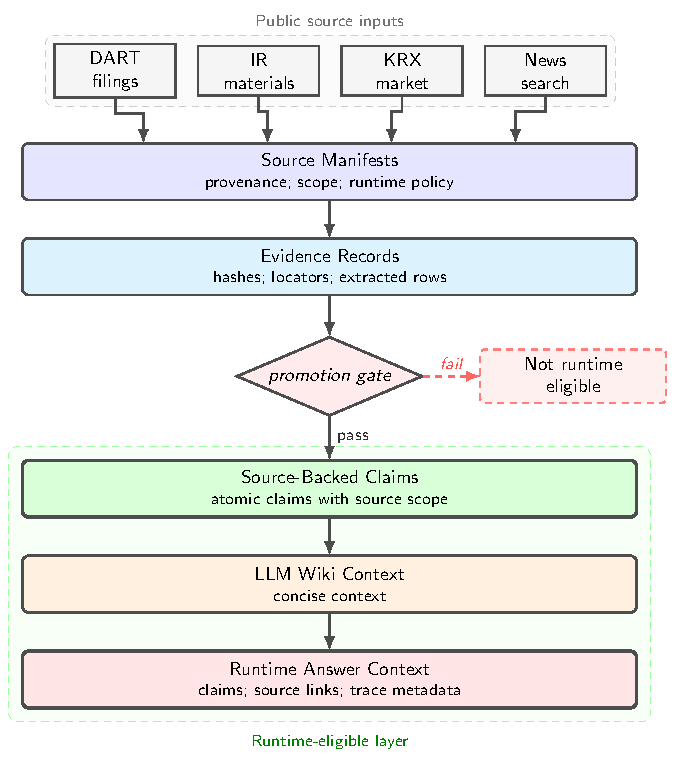
\includegraphics[width=0.95\linewidth,height=0.62\textheight,keepaspectratio]{figures/source_to_claim_pipeline.pdf}
    \caption{Source-to-claim pipeline. DART filings, issuer IR materials, KRX market rows, and news-search results are registered as source manifests before they are promoted as source-backed claims or attached as traceable runtime signals.}
    \label{fig:source-to-claim}
\end{figure}

\subsection{Runtime Claim Layer}

The source-backed runtime layer used in the case study is summarized in \Cref{tab:data-artifacts}. Runtime claims are the promoted, source-backed statements that the answer composer is allowed to use at runtime. They are distinct from raw document counts, extracted sentence counts, and company-importance measures. The claim counts are intentionally smaller than the number of collected files because they count only statements that passed source-linking and runtime-promotion gates. Differences across corporate groups reflect how many source-backed statements were promoted for the current fixed validation scenarios and answer templates.

The counts exclude downloaded files, extracted text, wiki pages, and unpromoted claim candidates. Most promoted claims in this baseline come from OpenDART records and selected official IR materials; market and news inputs are handled as runtime signals.

The five-corporate-group manifests currently contain 113 source-backed runtime claims. A compact 25-claim review-selected reference layer, five priority claims per corporate group, is used for paper reporting and product inspection. The 25-claim layer keeps reported coverage tied to selected evidence while still making transfer progress measurable: the ledger documents the wider source inventory, while the runtime layer uses only promoted, source-linked claims.

\begin{table}[H]
    \centering
    \caption{Source-backed runtime claim layer in the reference implementation.}
    \label{tab:data-artifacts}
    \footnotesize
    \setlength{\tabcolsep}{3pt}
    \renewcommand{\arraystretch}{1.25}
    \begin{tabular}{@{}C{0.15\linewidth}
                    C{0.13\linewidth}
                    L{0.31\linewidth}
                    L{0.29\linewidth}@{}}
        \toprule
        \multicolumn{1}{C{0.15\linewidth}}{Corporate group} & \multicolumn{1}{C{0.13\linewidth}}{Runtime claims} & \multicolumn{1}{C{0.31\linewidth}}{Claim coverage} & \multicolumn{1}{C{0.29\linewidth}}{Validation role} \\
        \midrule
        Samsung & 36 & Memory/electronics, battery, construction, bio, components & Tests routing across the broadest affiliate mix in the slice \\
        \addlinespace[0.35em]
        SK & 27 & Memory, energy, holding-company, telecom, ICT investment & Tests semiconductor and portfolio-allocation questions \\
        \addlinespace[0.35em]
        Hyundai Motor & 15 & OEMs, parts, logistics, defense/rail & Tests mobility-centered affiliate routing and source separation \\
        \addlinespace[0.35em]
        LG & 15 & Electronics, materials, battery, components, telecom & Tests electronics-battery-materials coverage with telecom cash-flow context \\
        \addlinespace[0.35em]
        Hanwha & 20 & Holding, aerospace, energy, systems, shipbuilding & Tests defense, energy, and shipbuilding claims under one corporate-group boundary \\
        \bottomrule
    \end{tabular}
\end{table}
\FloatBarrier

\PostFigureHeadingSpace
\section{System Validation Results}

This section evaluates whether the reconstructed system preserves its operating contracts in the bounded reference slice. The validation checks whether source grounding, routing, trace completeness, output hygiene, interface connectivity, and latency remain under engineering control.

\subsection{Validation Protocol}

Each fixed validation scenario is a versioned test case: one investor-facing question, an entity scope, expected claims, required answer signals, trace requirements, prohibited patterns, and a latency budget. It passes only when all required evidence and trace fields resolve and no configured blocker fires.
The scenario questions are product-facing briefing prompts, not expert-approved investment recommendations. Some prompts use terms such as investment point because the motivating demonstration needed questions that were recognizable to business users; in this paper, those prompts test routing, evidence selection, answer structure, and trace preservation.

The role of each contract area is defined in \Cref{tab:enterprise-validation-frame}. Prompt, model, and output evaluation tools measure important application behavior; the reconstructed architecture adds a product-control layer for source authority, entity scope, trace retention, and user-facing constraints.

\begin{table}[H]
    \centering
    \caption{Contract frame for system-level assessment.}
    \label{tab:enterprise-validation-frame}
    \footnotesize
    \setlength{\tabcolsep}{4pt}
    \renewcommand{\arraystretch}{1.20}
    \begin{tabular}{@{}C{0.20\linewidth}
                    L{0.39\linewidth}
                    L{0.31\linewidth}@{}}
        \toprule
        \multicolumn{1}{C{0.20\linewidth}}{Contract area} & \multicolumn{1}{C{0.39\linewidth}}{Requirement} & \multicolumn{1}{C{0.31\linewidth}}{Evidence reported} \\
        \midrule
        Source grounding & Runtime answers must remain tied to registered sources and promoted claims. & Claim-reference and trace-field outcomes in \Cref{tab:validation-results}. \\
        Entity and answer scope & Fixed scenarios must preserve entity scope, required answer signals, and prohibited-language constraints. & Scenario outcomes in \Cref{tab:validation-results} and the fault-injection sensitivity check in \Cref{sec:fault-injection-sensitivity}. \\
        Output hygiene & User-facing answers must stay separated from internal traces while preserving source links and answer structure. & Answer and gate outcomes in \Cref{tab:validation-results}. \\
        Runtime interfaces & Live interfaces and orchestration should connect to external sources while preserving the answer contract. & Live-interface outcomes in \Cref{sec:runtime-interfaces}; latency outcomes in \Cref{tab:latency-results}. \\
        \bottomrule
    \end{tabular}
\end{table}

The fixed validation slice contains 30 investor-facing scenarios: five selected-company questions and one cross-company comparison for each of the five corporate-group slices. Appendix~\ref{app:scenario-inventory} gives the scenario inventory, question-design rules, and representative question examples.

\subsection{Scenario Contract Outcomes}

Fixed validation scenarios test whether the system preserves its source, routing, trace, and answer-structure contracts. They are narrower than full RAG evaluation \citep{es2023ragas,saadfalcon2024ares,liang2023helm}; their role is to fix a reproducible baseline for contract preservation. The aggregate outcomes for the six fixed questions per corporate group are reported in \Cref{tab:validation-results}. Each corporate group uses the same question design: five selected-company questions plus one cross-company comparison. Each result cell reports passing configured checks over required checks.

\vspace{-0.25\baselineskip}
\begin{table}[!htbp]
    \centering
    \caption{Fixed validation-scenario contract results.}
    \label{tab:validation-results}
    \footnotesize
    \setlength{\tabcolsep}{6pt}
    \renewcommand{\arraystretch}{1.12}
    \begin{tabular*}{0.98\linewidth}{@{\extracolsep{\fill}}C{0.20\linewidth}cccccc@{}}
        \toprule
        \multicolumn{1}{C{0.20\linewidth}}{Corporate group} & Scenarios & Claim refs & Trace & Answer & Hygiene & Failed \\
        \midrule
        Samsung & 6/6 & 25/25 & 6/6 & 6/6 & 12/12 & 0 \\
        SK & 6/6 & 30/30 & 6/6 & 6/6 & 12/12 & 0 \\
        Hyundai Motor & 6/6 & 20/20 & 6/6 & 6/6 & 12/12 & 0 \\
        LG & 6/6 & 20/20 & 6/6 & 6/6 & 12/12 & 0 \\
        Hanwha & 6/6 & 14/14 & 6/6 & 6/6 & 12/12 & 0 \\
        \midrule
        Total & 30/30 & 109/109 & 30/30 & 30/30 & 60/60 & 0 \\
        \bottomrule
    \end{tabular*}
    \vspace{0.10em}
    \begin{minipage}{0.94\linewidth}
        \footnotesize
        Cells report passed checks over required checks. \textit{Claim refs} counts expected source-backed claim references. \textit{Trace}, \textit{Answer}, and \textit{Hygiene} check the audit envelope, visible answer contract, and leakage/link controls.
    \end{minipage}
\end{table}
\vspace{-0.35\baselineskip}

Within the bounded reference slice, all configured source, trace, answer, and output-hygiene contracts passed. The 109/109 source-claim result means that every expected evidence reference in the scenario files resolved to a promoted claim. The 30/30 trace-contract result means that every answer preserved the required audit envelope. The 30/30 answer-contract result means that every visible answer contained the required answer signals and avoided prohibited patterns. The 60/60 output-hygiene result means that internal-trace leakage was blocked and user-visible source links were preserved across the 30 scenarios. The 0 failed runs result means that no scenario was stopped by a configured blocker. The corresponding evaluator artifacts are stored in the repository's \path{evals/results/} directory.

The user-facing answer view associated with these checks is shown in \Cref{fig:ui-mobile-answer}. The visible answer summarizes financial metrics, risks, and monitoring points while keeping comparative items bounded by the answer contract. The source-link and follow-up region is shown in \Cref{fig:representative-answer-output}.

\begin{figure}[H]
    \centering
    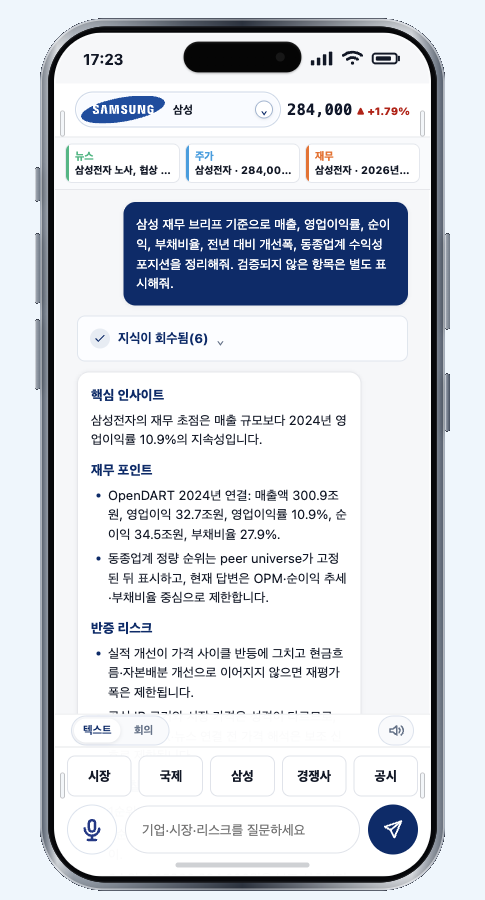
\includegraphics[width=0.49\linewidth]{figures/ui_mobile_answer_ko.png}
    \caption{Mobile answer view for a fixed finance-brief scenario. The retrieved-knowledge marker denotes a loaded evidence package; the answer uses insight-first sections with internal trace artifacts kept in the audit layer.}
    \label{fig:ui-mobile-answer}
\end{figure}

\subsection{Fault-Injection Sensitivity}
\label{sec:fault-injection-sensitivity}

Here, fault injection refers to mutating one contract property at a time to test validator sensitivity. Starting from one valid scenario, seven mutated copies were evaluated with the same contract checks. The validator detected all seven induced violations and missed none. The concrete mutation protocol is shown in \Cref{tab:fault-injection-protocol}, and the full artifact is stored under the repository's \path{evals/results/} directory. When key contract properties are deliberately broken, the corresponding validators fail the run.

\subsection{Runtime Interfaces and Orchestration}
\label{sec:runtime-interfaces}

After fixed-scenario validation, the implementation was exercised with live filing, market, and news interfaces. Runtime interface checks passed 5/5 live API corporate-group connectivity checks and 15/15 live answer-hygiene checks, with inspection packets generated for all 15 runtime samples. These checks verify interface wiring and artifact hygiene.

Latency was measured on the 14 scenarios that had paired baseline and optimized measurements in the May 3 latency dashboard. The optimized run used parallel source collection and process-level caching for repeated source reads. As shown in \Cref{tab:latency-results}, mean latency decreased from 2008.57ms to 171.14ms, and the number of runs under the fixed 1500ms engineering budget increased from 2/14 to 13/14. The budget is used as an internal runtime threshold for these fixed scenarios. The measurements use the deterministic composer; live-LLM provider latency is outside this comparison. These results show that the same answer contract can be preserved while the runtime moves from static artifacts toward live source interfaces and optimized orchestration.

\begin{table}[!htbp]
    \centering
    \caption{Fixed-scenario latency before and after runtime optimization.}
    \label{tab:latency-results}
    \footnotesize
    \renewcommand{\arraystretch}{1.12}
    \begin{tabular*}{0.96\linewidth}{@{\extracolsep{\fill}}C{0.31\linewidth}C{0.25\linewidth}C{0.25\linewidth}@{}}
        \toprule
        \multicolumn{1}{C{0.31\linewidth}}{Measure} & \multicolumn{1}{C{0.25\linewidth}}{Baseline run} & \multicolumn{1}{C{0.25\linewidth}}{Optimized run} \\
        \midrule
        Scenario count & 14 & 14 \\
        Average latency & 2008.57ms & 171.14ms \\
        Median latency & 2156ms & 86ms \\
        p90 latency & 2467ms & 143ms \\
        Runs under 1500ms budget & 2/14 & 13/14 \\
        \bottomrule
    \end{tabular*}
\end{table}

\PostTableHeadingSpace
\section{Discussion}

The validation results characterize the implemented architecture at the systems-engineering layer. In the bounded public-data slice, source grounding, entity routing, answer structure, trace generation, and output hygiene are represented as explicit artifacts and exercised through repeatable checks. The discussion below explains what this means for productization and reproducibility.

\subsection{Engineering Interpretation}

The reconstruction changes the unit of control from prompt instructions to versioned engineering artifacts. The motivating PoC surfaced a productization pattern in which useful behavior appeared before the system had explicit source, trace, and validation contracts. In the reconstructed system, source manifests, company-scoped claims, code-owned routing, answer contracts, and validation traces govern the answer process. This approach is complementary to prompt engineering: prompts still guide language behavior, while the surrounding architecture assigns ownership for evidence boundaries, entity scope, output structure, leakage prevention, and inspection.

The proposed pattern also differs from adjacent engineering approaches in emphasis. DSPy-style program optimization focuses on compiling and optimizing language-model pipelines \citep{khattab2024dspy}, while MLOps addresses broader lifecycle deployment concerns \citep{kreuzberger2023mlops}. The architecture described here is narrower: it defines how a generated enterprise answer remains connected to source manifests, source-backed claims, routing metadata, answer contracts, and traces. This distinction matters because enterprise readers need a useful answer, while developers and researchers need a separate trace that explains how the answer was assembled.

The results have three implications for the implemented system. First, the fixed validation-scenario runs show that expected source, routing, trace, and answer-structure contracts were preserved across the reference slice. Second, the fault-injection results show that the validators detected deliberately broken source, routing, trace, answer, leakage, link, and latency conditions. Third, the latency result shows that orchestration and caching improved runtime behavior and preserved the answer contract. The latency result is an operational signal; the broader contribution is the architecture-level separation of sources, claims, routing, answer contracts, traces, and validation gates.

\subsection{Productization Implications}
\label{sec:reproducibility}
\enlargethispage{3\baselineskip}

In practitioner discussions, organizations often ask how to locate their current AI-agent adoption state before full deployment. The harness becomes useful when product behavior must move from plausible interaction to governed operation: source scope, entity routing, claim eligibility, answer contracts, and traces become explicit organizational capabilities. \Cref{tab:maturity-ladder} translates that productization need into a descriptive adoption framework: Level 1 is prompt-centered, while Level 5 represents a traceable system with governed evidence and validation artifacts. The framework supports planning; scoring a particular organization remains a separate assessment.

\begin{table}[H]
    \centering
    \caption{Descriptive adoption framework for enterprise LLM-agent systems.}
    \label{tab:maturity-ladder}
    \footnotesize
    \renewcommand{\arraystretch}{1.12}
    \begin{tabular}{C{0.12\linewidth} L{0.32\linewidth} L{0.44\linewidth}}
        \toprule
        \multicolumn{1}{C{0.12\linewidth}}{Level} & \multicolumn{1}{C{0.32\linewidth}}{System state} & \multicolumn{1}{C{0.44\linewidth}}{Observable capability} \\
        \midrule
        1 & Prompt-centered chatbot & Product behavior is mainly controlled by instructions; source scope and validation remain informal. \\
        2 & RAG-based assistant & Retrieved documents support answers; evidence boundaries and traces are still partial. \\
        3 & Source-manifest system & Approved sources are registered with scope, URLs, update metadata, and ownership. \\
        4 & Claim-governed agent & Runtime claims, entity routing, and evidence states govern answer assembly. \\
        5 & Traceable harness & Answers, source links, validation results, and audit traces are versioned and can be replayed in validation runs. \\
        \bottomrule
    \end{tabular}
\end{table}

Applied to a new enterprise target, the pattern requires a concrete source and claim package. Public or client-approved sources must be registered, source-backed claims promoted, routing rules checked, and scenario contracts run. The public-data baseline makes these steps inspectable before private documents, production credentials, or operational logs are introduced. The framework also separates system readiness from usefulness for investment analysis: this paper evaluates preservation of source, routing, answer, trace, and hygiene contracts, while expert review and deployment evidence are left to later domain-value evaluation.

The reproducible layer consists of scenario JSON files, source and claim manifests, validation scripts, sanitized traces, and fixture or smoke-test modes. At public submission, the release package will record the public repository URL and commit hash for the submitted baseline; the current manuscript keeps this as a replaceable repository placeholder \citep{ahnkim2026advisorrepo}. Some materials cannot be redistributed directly: API keys, copyrighted PDFs, and future client-operation logs must remain private. For those materials, the reproducibility strategy provides public URLs, source manifests, checksums when available, evidence records, and claim manifests as redistributable metadata. Until the release repository is public, code and sanitized artifacts are available from the corresponding author upon request.

\section{Conclusion}

This paper has shown how a prompt-dominant enterprise LLM proof-of-concept can be reconstructed as a traceable LLM-agent architecture. By moving source gates, claim layers, routing metadata, answer contracts, and validation traces into explicit harness artifacts, the implementation makes enterprise behavior more inspectable while retaining evidence for audit and reproduction.

The reference implementation applies the approach to a bounded 25-company public-data slice across five Korean corporate groups. The system-level validation checks traceability, routing, migration from prompt rules to code, prevention of internal-output leakage, runtime-interface behavior, and latency. The latency result is one operational signal; the broader contribution is that enterprise behavior is relocated from an expanding prompt into artifacts that can be inspected, versioned, tested, and extended.

Future work can broaden source coverage, add larger runtime ablations and expert review, harden live interfaces, and evaluate whether the briefings support professional investment analysis. A subsequent deployment study can compare the submitted baseline against commercialized versions with operational logs and live-LLM runs. One lesson from the case study is that enterprise LLM productization combines modeling concerns with systems-engineering concerns: the model must be surrounded by explicit source gates, runtime contracts, validation traces, and inspection surfaces before it is extended in commercial settings.


\section*{Disclosures}

The study uses public and official materials only. The named corporate groups are included as a public-data engineering slice and had no sponsorship role in the study. The motivating prototype was developed during a CEO AI program, and the AI Leadership Research Center affiliation reflects the CEO AI program context; CEO AI provided no funding for the paper, and the named corporate groups had no role in study design or reporting. The system is designed for traceable briefing and source inspection, with investment-advice and investment-performance evaluation outside the study scope. Live-LLM run requirements and repository availability are described in \Cref{sec:implementation-details,sec:reproducibility}.

\appendix
\raggedbottom
\section*{Appendix}
\renewcommand{\thesubsection}{A\arabic{subsection}}
\renewcommand{\thetable}{A\arabic{table}}
\renewcommand{\thefigure}{A\arabic{figure}}
\setcounter{subsection}{0}
\setcounter{table}{0}
\setcounter{figure}{0}
This appendix documents the 30 fixed validation questions underlying \Cref{tab:validation-results}. The set covers five Korean corporate groups, with six questions per group: five selected-company briefings and one cross-company comparison. The versioned JSON artifacts retain the Korean prompts, expected claims, routing expectations, and answer checks.

\subsection{Validation Scenario Set}
\label{app:scenario-inventory}

The question design for each corporate group is summarized in \Cref{tab:question-design}.

\begingroup
\footnotesize
\setlength{\tabcolsep}{3pt}
\renewcommand{\arraystretch}{1.12}
\begin{longtable}{@{}C{0.12\linewidth}
                L{0.34\linewidth}
                L{0.25\linewidth}
                L{0.20\linewidth}@{}}
    \caption{Fixed validation-question design by corporate group.}
    \label{tab:question-design}\\
    \toprule
    \multicolumn{1}{C{0.12\linewidth}}{Corporate group} & \multicolumn{1}{C{0.34\linewidth}}{Differentiated question focus} & \multicolumn{1}{C{0.25\linewidth}}{Permitted evidence scope} & \multicolumn{1}{C{0.20\linewidth}}{Validation purpose} \\
    \midrule
    \endfirsthead
    \caption[]{Fixed validation-question design by corporate group (continued).}\\
    \toprule
    \multicolumn{1}{C{0.12\linewidth}}{Corporate group} & \multicolumn{1}{C{0.34\linewidth}}{Differentiated question focus} & \multicolumn{1}{C{0.25\linewidth}}{Permitted evidence scope} & \multicolumn{1}{C{0.20\linewidth}}{Validation purpose} \\
    \midrule
    \endhead
    \midrule
    \multicolumn{4}{r}{Continued on next page}\\
    \endfoot
    \bottomrule
    \endlastfoot
    Samsung & Semiconductor recovery, battery profitability, shareholder letter, biologics orders, insurance capital/dividend, and electronics--battery comparison. & DART financial data; official IR/DART narratives; financial affiliates limited to capital and dividend evidence. & Tests separation across electronics, battery, bio, construction, and financial-company evidence. \\
    SK & AI memory, battery restructuring, holding-company value-up, telecom AI/data centers, SK Square NAV/shareholder return, and Hynix--Innovation comparison. & DART financial data; value-up and shareholder-return material; source-backed operating-company and holding-company strategy claims. & Tests separation between operating-company, holding-company, and investment-company evidence. \\
    Hyundai Motor & Automaker, parts, logistics, defense/rail, and Hyundai Motor--Kia financial comparison questions. & DART annual financial data and business-mix claims tied to mobility and supply-chain affiliates. & Tests affiliate routing inside a closely related industrial supply chain. \\
    LG & Electronics, chemicals, battery, components, telecom financial trends, and electronics--chemicals comparison. & DART annual financial data and source-backed business-driver claims for heterogeneous sectors. & Tests whether the shared schema transfers across heterogeneous industries. \\
    Hanwha & Holding-company, aerospace, solar/materials, defense electronics, shipbuilding, and aerospace--solutions comparison questions. & DART financial data; official IR narratives; market and news interfaces only as traceable runtime signals when available. & Tests evidence contracts across defense, energy, systems, and shipbuilding topics. \\
\end{longtable}
\endgroup

Each group uses six questions: five selected-company briefings and one cross-company comparison. The columns specify question focus, permitted evidence scope, and validation purpose; a scenario set passes when routing, required claims, source links, follow-ups, and hidden-trace controls pass for all six questions. The prompts are translated for readability, with the original Korean prompts and expected claims stored in the scenario JSON files.

The table records design intent and links each question focus to the contract outcomes reported in \Cref{tab:validation-results}. Representative translated prompts are shown in \Cref{tab:question-examples}; the examples include briefing cards, market and filing signals, source links, follow-up questions, and bounded comparisons.

\subsection{Representative Question Examples}
\label{app:question-examples}

Translated examples of the fixed validation questions are given in \Cref{tab:question-examples}. The exact Korean prompts are stored in the versioned scenario JSON files. The examples vary the surface being exercised: news, market, filing, answer support, and bounded comparison.

\begingroup
\scriptsize
\setlength{\tabcolsep}{3pt}
\renewcommand{\arraystretch}{1.12}
\begin{longtable}{@{}C{0.19\linewidth}
                L{0.50\linewidth}
                L{0.22\linewidth}@{}}
    \caption{Representative fixed validation-scenario question examples.}
    \label{tab:question-examples}\\
    \toprule
    \multicolumn{1}{C{0.19\linewidth}}{Example type} & \multicolumn{1}{C{0.50\linewidth}}{Translated example question} & \multicolumn{1}{C{0.22\linewidth}}{Contract focus} \\
    \midrule
    \endfirsthead
    \caption[]{Representative fixed validation-scenario question examples (continued).}\\
    \toprule
    \multicolumn{1}{C{0.19\linewidth}}{Example type} & \multicolumn{1}{C{0.50\linewidth}}{Translated example question} & \multicolumn{1}{C{0.22\linewidth}}{Contract focus} \\
    \midrule
    \endhead
    \midrule
    \multicolumn{3}{r}{Continued on next page}\\
    \endfoot
    \bottomrule
    \endlastfoot
    Samsung selected company & Separate Samsung Electronics news, stock, and filing signals, then state what each source supports. & News, market, and filing separation \\
    SK selected company & Explain how the SK Hynix AI-memory brief is grounded and which follow-ups should be offered. & Affiliate routing and follow-up filtering \\
    Hyundai Motor selected company & Distinguish Hyundai Motor price movement from operating-performance evidence. & Market signal and filing evidence separation \\
    LG selected company & Summarize the LG Energy Solution battery-sector brief with source links and no unsupported forecast. & Source-link preservation and forecast restraint \\
    Hanwha selected company & Separate Hanwha Aerospace news and disclosure evidence before generating follow-up questions. & Evidence boundary and follow-up generation \\
    Cross-company comparison & Compare Hanwha Aerospace and Hanwha Solutions within promoted claims and source links. & Multi-entity routing and bounded comparison \\
    Answer-support check & After a finance brief, list source links and follow-up questions for reader inspection. & Reader-facing support controls \\
\end{longtable}
\endgroup

\subsection{Answer-Level Contract Examples}
\label{app:answer-contract-example}

The visible answer is part of the checked artifact. \Cref{tab:representative-answer-contract} summarizes representative output signals without reproducing full Korean transcripts; aggregate pass counts remain in \Cref{tab:validation-results}. Source links and follow-up questions are shown in \Cref{fig:representative-answer-output}.

\begingroup
\footnotesize
\setlength{\tabcolsep}{3pt}
\renewcommand{\arraystretch}{1.12}
\begin{longtable}{@{}C{0.12\linewidth}
                L{0.40\linewidth}
                L{0.24\linewidth}
                L{0.16\linewidth}@{}}
    \caption{Representative reader-visible answer signals across product surfaces.}
    \label{tab:representative-answer-contract}\\
    \toprule
    \multicolumn{1}{C{0.12\linewidth}}{Group} & \multicolumn{1}{C{0.40\linewidth}}{Representative visible output} & \multicolumn{1}{C{0.24\linewidth}}{Reader-facing support} & \multicolumn{1}{C{0.16\linewidth}}{Follow-up direction} \\
    \midrule
    \endfirsthead
    \caption[]{Representative reader-visible answer signals across product surfaces (continued).}\\
    \toprule
    \multicolumn{1}{C{0.12\linewidth}}{Group} & \multicolumn{1}{C{0.40\linewidth}}{Representative visible output} & \multicolumn{1}{C{0.24\linewidth}}{Reader-facing support} & \multicolumn{1}{C{0.16\linewidth}}{Follow-up direction} \\
    \midrule
    \endhead
    \midrule
    \multicolumn{4}{r}{Continued on next page}\\
    \endfoot
    \bottomrule
    \endlastfoot
    Samsung & Finance brief foregrounds margin recovery: 2024 revenue KRW 300.9T, operating income KRW 32.7T, and OPM 10.9\%; market-price evidence stays in the stock card. & DART filing, IR/filing package, KRX row, and news link remain visible to the reader. & Margin durability; debt and cash flow; shareholder return. \\
    SK & The visible answer separates SK Hynix AI-memory recovery from holding-company and investment-company questions, flagging HBM premium, CAPEX, and customer concentration as distinct variables. & Filing and IR links are exposed with selected claim evidence and source-state labels. & HBM CAPEX; customer exposure; SK Square NAV. \\
    Hyundai Motor & The output keeps stock movement as a market signal and operating performance as filing evidence, with sales mix, foreign exchange, hybrid/EV transition, and shareholder return treated as separate briefing axes. & KRX price row, OpenDART financial rows, and source links are shown as separate reader controls. & Hyundai--Kia comparison; margin resilience; parts and electrification. \\
    LG & The answer frames electronics cash flow separately from battery and chemical-cycle recovery, so margin defense and recovery timing are not collapsed into a single group-level statement. & OpenDART rows, IR/DART links, market rows, and unavailable-source states are labeled. & Battery cycle; LG Electronics margin; LG Chem recovery. \\
    Hanwha & Cross-company answers preserve the selected entities: aerospace, energy/materials, systems, and shipbuilding evidence are kept in bounded comparison rather than merged into one generic group brief. & DART, official IR, news, and market links are exposed where available with source-state labels. & Aerospace vs. Solutions; rights-issue evidence; disclosure risk signals. \\
\end{longtable}
\noindent These examples are condensed from generated answers: the table records the reader-visible signal, supporting evidence, and follow-up direction checked by the contract, while the full Korean answer text remains in the generated artifact.
\endgroup

\begin{figure}[H]
    \centering
    \makebox[\textwidth][c]{%
    \begin{minipage}[t]{0.49\linewidth}
        \centering
        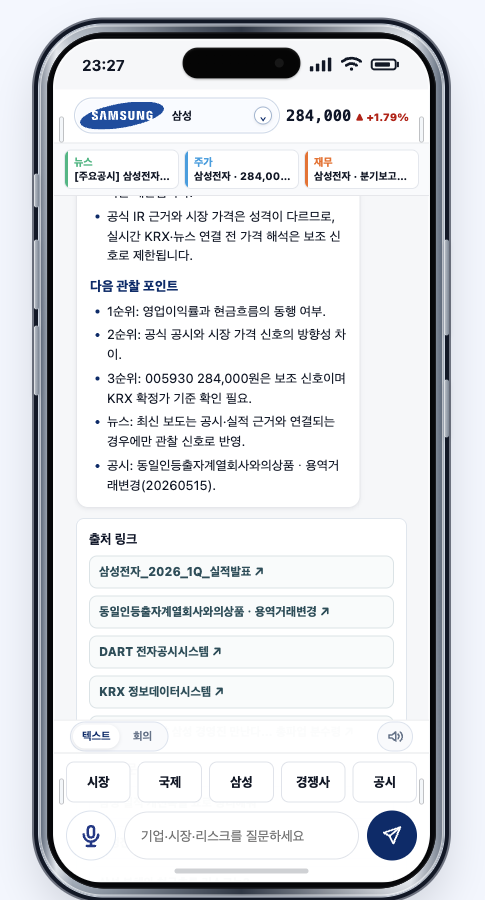
\includegraphics[width=\linewidth]{figures/ui_mobile_sources_ko.png}\\[-0.25em]
        {\small (a) Source links.}
    \end{minipage}
    \hspace{0.015\linewidth}
    \begin{minipage}[t]{0.49\linewidth}
        \centering
        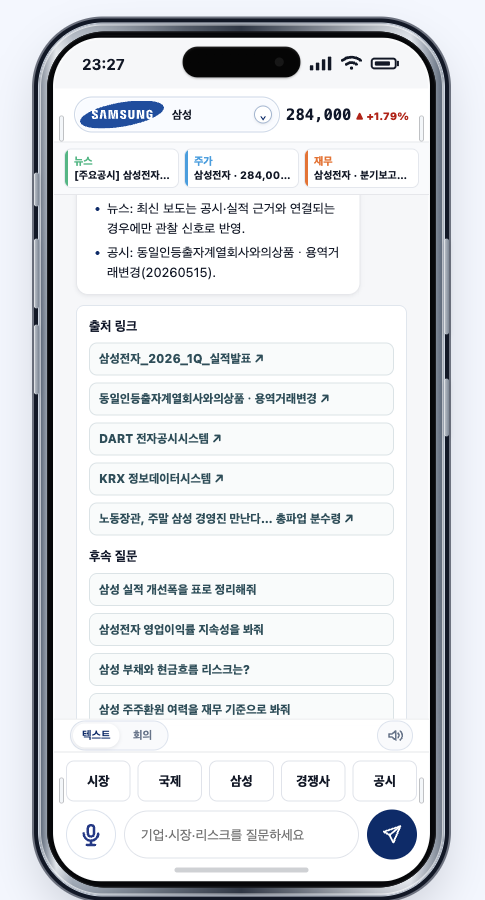
\includegraphics[width=\linewidth]{figures/ui_mobile_followups_ko.png}\\[-0.25em]
        {\small (b) Follow-up questions.}
    \end{minipage}}
    \caption{Representative answer-support screens in full mobile context. Panel (a) shows reader-facing source links; panel (b) shows generated follow-up questions, with internal trace details kept out of the visible answer.}
    \label{fig:representative-answer-output}
\end{figure}

\FloatBarrier

\subsection{Fault-Injection Protocol}
\label{app:fault-injection-protocol}

The fault-injection check induced seven contract violations, all of which were detected. \Cref{tab:fault-injection-protocol} lists the mutation rule and detected validator; the full JSON artifact is stored in \path{evals/results/} \citep{ahnkim2026advisorrepo}.

\begin{table}[H]
    \centering
    \small
    \setlength{\tabcolsep}{3pt}
    \renewcommand{\arraystretch}{1.12}
    \caption{Concrete mutation protocol for the fault-injection check.}
    \label{tab:fault-injection-protocol}
    \begin{tabular}{@{}C{0.18\linewidth}
                    L{0.25\linewidth}
                    L{0.37\linewidth}
                    C{0.13\linewidth}@{}}
    \toprule
    \multicolumn{1}{C{0.18\linewidth}}{Contract dimension} & \multicolumn{1}{C{0.25\linewidth}}{Baseline field mutated} & \multicolumn{1}{C{0.37\linewidth}}{Injected violation} & \multicolumn{1}{C{0.13\linewidth}}{Detected validator} \\
    \midrule
    Source claims & \path{sourceClaims} & Remove expected claim \texttt{samsung-sbc-020} from the source-claim package. & Claim coverage \\
    \bottomrule
    \end{tabular}
\end{table}

\begin{table}[H]
    \ContinuedFloat
    \centering
    \small
    \setlength{\tabcolsep}{3pt}
    \renewcommand{\arraystretch}{1.12}
    \caption[]{Concrete mutation protocol for the fault-injection check (continued).}
    \begin{tabular}{@{}C{0.18\linewidth}
                    L{0.25\linewidth}
                    L{0.37\linewidth}
                    C{0.13\linewidth}@{}}
    \toprule
    \multicolumn{1}{C{0.18\linewidth}}{Contract dimension} & \multicolumn{1}{C{0.25\linewidth}}{Baseline field mutated} & \multicolumn{1}{C{0.37\linewidth}}{Injected violation} & \multicolumn{1}{C{0.13\linewidth}}{Detected validator} \\
    \midrule
    Entity routing & \texttt{representative}\newline\texttt{CompanyId} and trace route & Replace \texttt{samsung-electronics} with an unrelated company identifier. & Trace contract \\
    Trace completeness & \path{trace.runId} & Delete a required trace field from the audit envelope. & Trace contract \\
    Answer contract & \path{answer} & Remove the required answer signal \textit{Samsung Electronics} from visible prose. & Answer contract \\
    Internal leakage & \path{answer} & Inject trace-schema labels and a raw source-claim identifier into the reader-facing answer. & Leakage gate \\
    Source links & \path{links[0].href} & Replace one source link with a non-resolving value, \texttt{not-a-valid-url}. & Link gate \\
    Latency budget & \path{elapsedMs} & Set elapsed time above the 1500ms pre-API latency budget. & Latency gate \\
    \bottomrule
    \end{tabular}
\end{table}


\PostReferencesSpace
\bibliographystyle{plainnat}
\bibliography{bib/references}

\end{document}
